%%%%%%%%%%%%%%%%%%%%%%%%%%%%%%%%%%%%%%%%%%%%%%%%%%%%%%%%%%%%%%%%
%%%%%%%%%%%%%%%%%%%%%%%%%%%%%%%%%%%%%%%%%%%%%%%%%%%%%%%%%%%%%%%%
%%%%
%%%% This text file is part of the source of 
%%%% `Introduction to High-Performance Scientific Computing'
%%%% by Victor Eijkhout, copyright 2012-2022
%%%%
%%%% This book is distributed under a Creative Commons Attribution 3.0
%%%% Unported (CC BY 3.0) license and made possible by funding from
%%%% The Saylor Foundation \url{http://www.saylor.org}.
%%%%
%%%% hpc_intro.tex : an appetite whetter
%%%%
%%%%%%%%%%%%%%%%%%%%%%%%%%%%%%%%%%%%%%%%%%%%%%%%%%%%%%%%%%%%%%%%
%%%%%%%%%%%%%%%%%%%%%%%%%%%%%%%%%%%%%%%%%%%%%%%%%%%%%%%%%%%%%%%%

\documentclass[11pt,headernav]{beamer}

\beamertemplatenavigationsymbolsempty
\usetheme{Madrid}%{Montpellier}
\usecolortheme{seahorse}
\setcounter{tocdepth}{1}

\usepackage{pslatex}
\usepackage{amsmath,multirow,multicol} %% load array before arydshln if you really need it

\setbeamertemplate{footline}{Eijkhout: HPC taste}

\newdimen\unitindent \unitindent=20pt
\usepackage[algo2e,noline,noend]{algorithm2e}

\def\sublocal{_{\mathrm\scriptstyle local}}

\usepackage{comment}

\input slidemacs
\input snippetmacs
\input scimacs

%\advance\textwidth by 1in
%\advance\oddsidemargin by -.5in

\begin{document}
\parskip=10pt plus 5pt minus 3pt

\title{A Taste of Scientific Computing}
\author{Victor Eijkhout}
\date{2022}

\begin{frame}
  \titlepage
\end{frame}

\begin{frame}\frametitle{What is Scientific Computing about?}
  You know the science; what more is there?
  \begin{itemize}
  \item Science often gives an implicit description.\\
    How do you turn it into something computational.
  \item Algorithms are not unique:\\
    There are many ways to solve a linear system
    \[ \mathop{?}_x\colon Ax=b \]
    What are pros and cons of the choices?
  \item Algorithms can be implemented multiple ways, depending on your
    processor.
  \end{itemize}
\end{frame}

\sectionframe{Algorithmic choices}

\begin{frame}{Summing forces}
  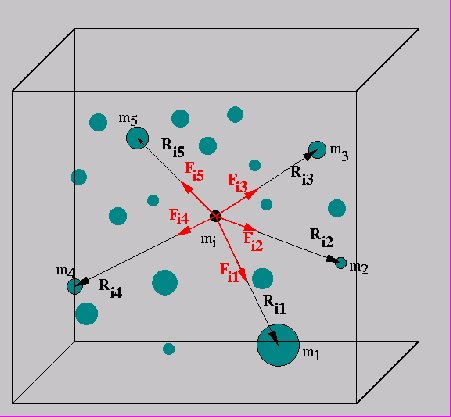
\includegraphics[scale=.45]{nbody_pic}
\end{frame}

\begin{frame}{Particle interactions}
  \begin{tabbing}
    for \=each particle $i$\\
    \>for \= each particle $j$\\
    \>\> let $\bar r_{ij}$ be the vector between $i$ and $j$;\\
    \>\> then the force on $i$ because of $j$ is\\
    \>\> $\quad f_{ij} = -\bar r_{ij}\frac{m_im_j}{|r_{ij}|}$\\
    \>\> (where $m_i,m_j$ are the masses or charges) and\\
    \>\> $f_{ji}=-f_{ij}$.
  \end{tabbing}
  Naive all-pairs algorithm: $O(N^2)$
\end{frame}

\begin{frame}
  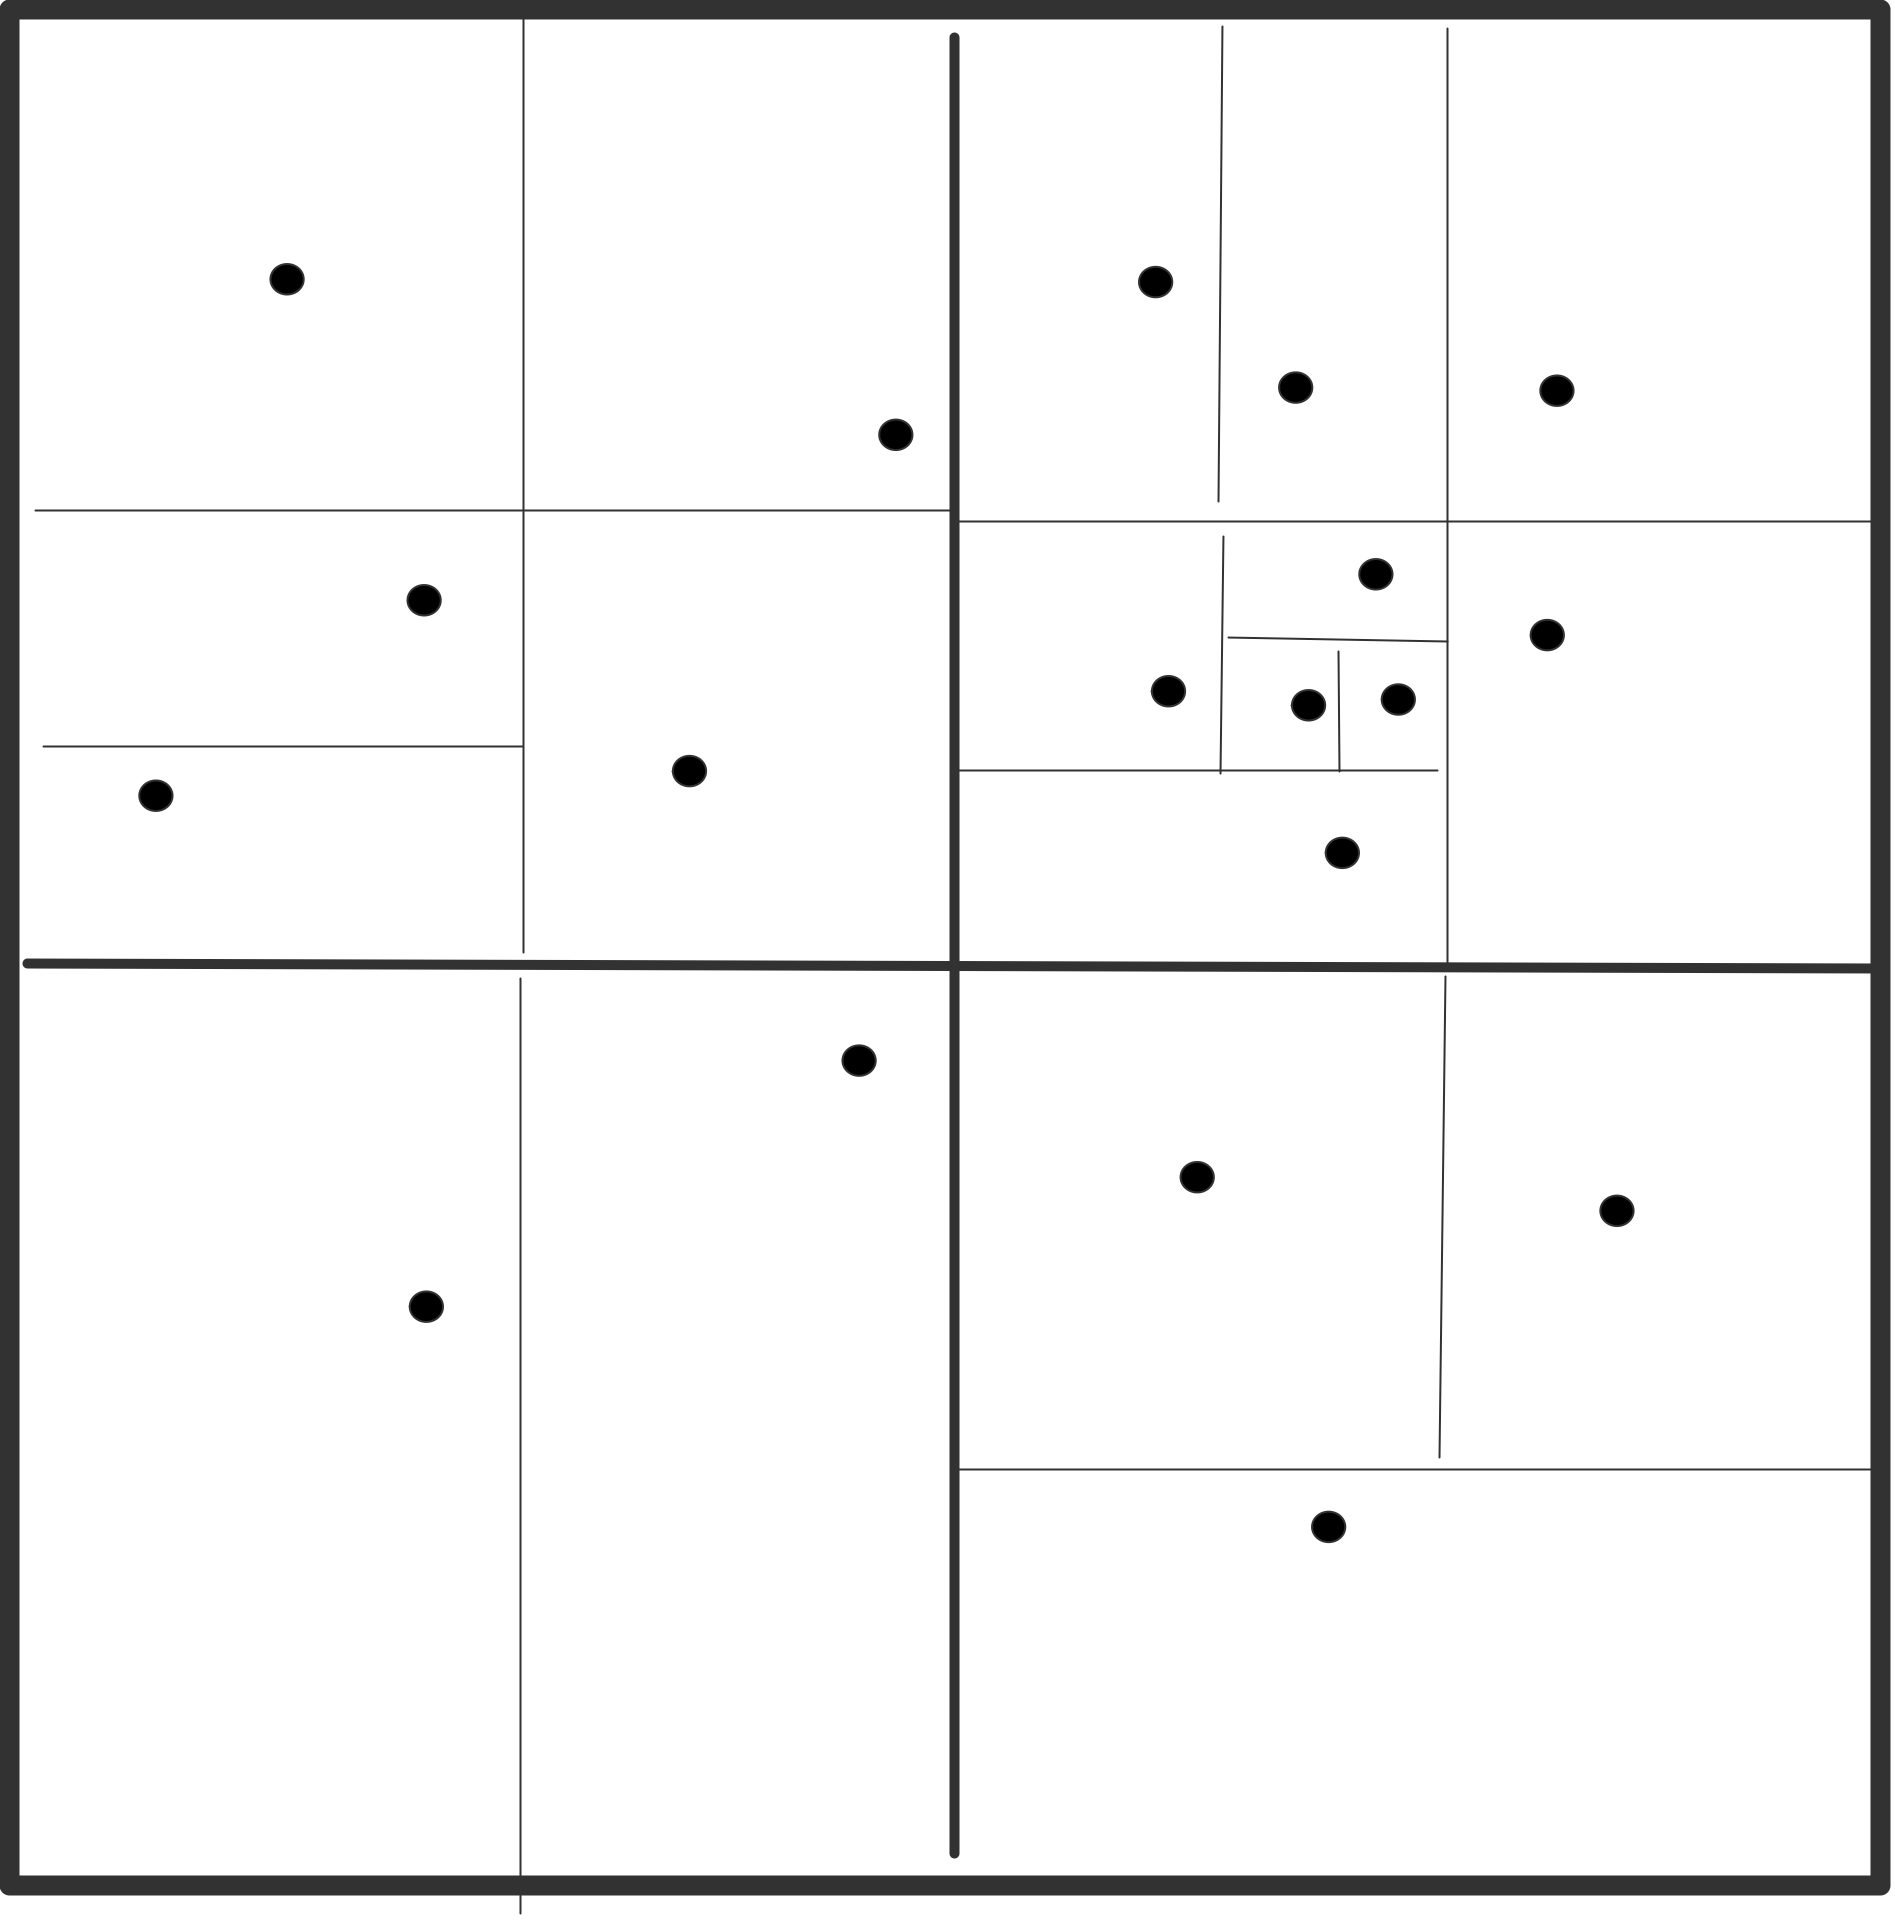
\includegraphics[scale=.08]{bh-quadrants-filled}
  %
  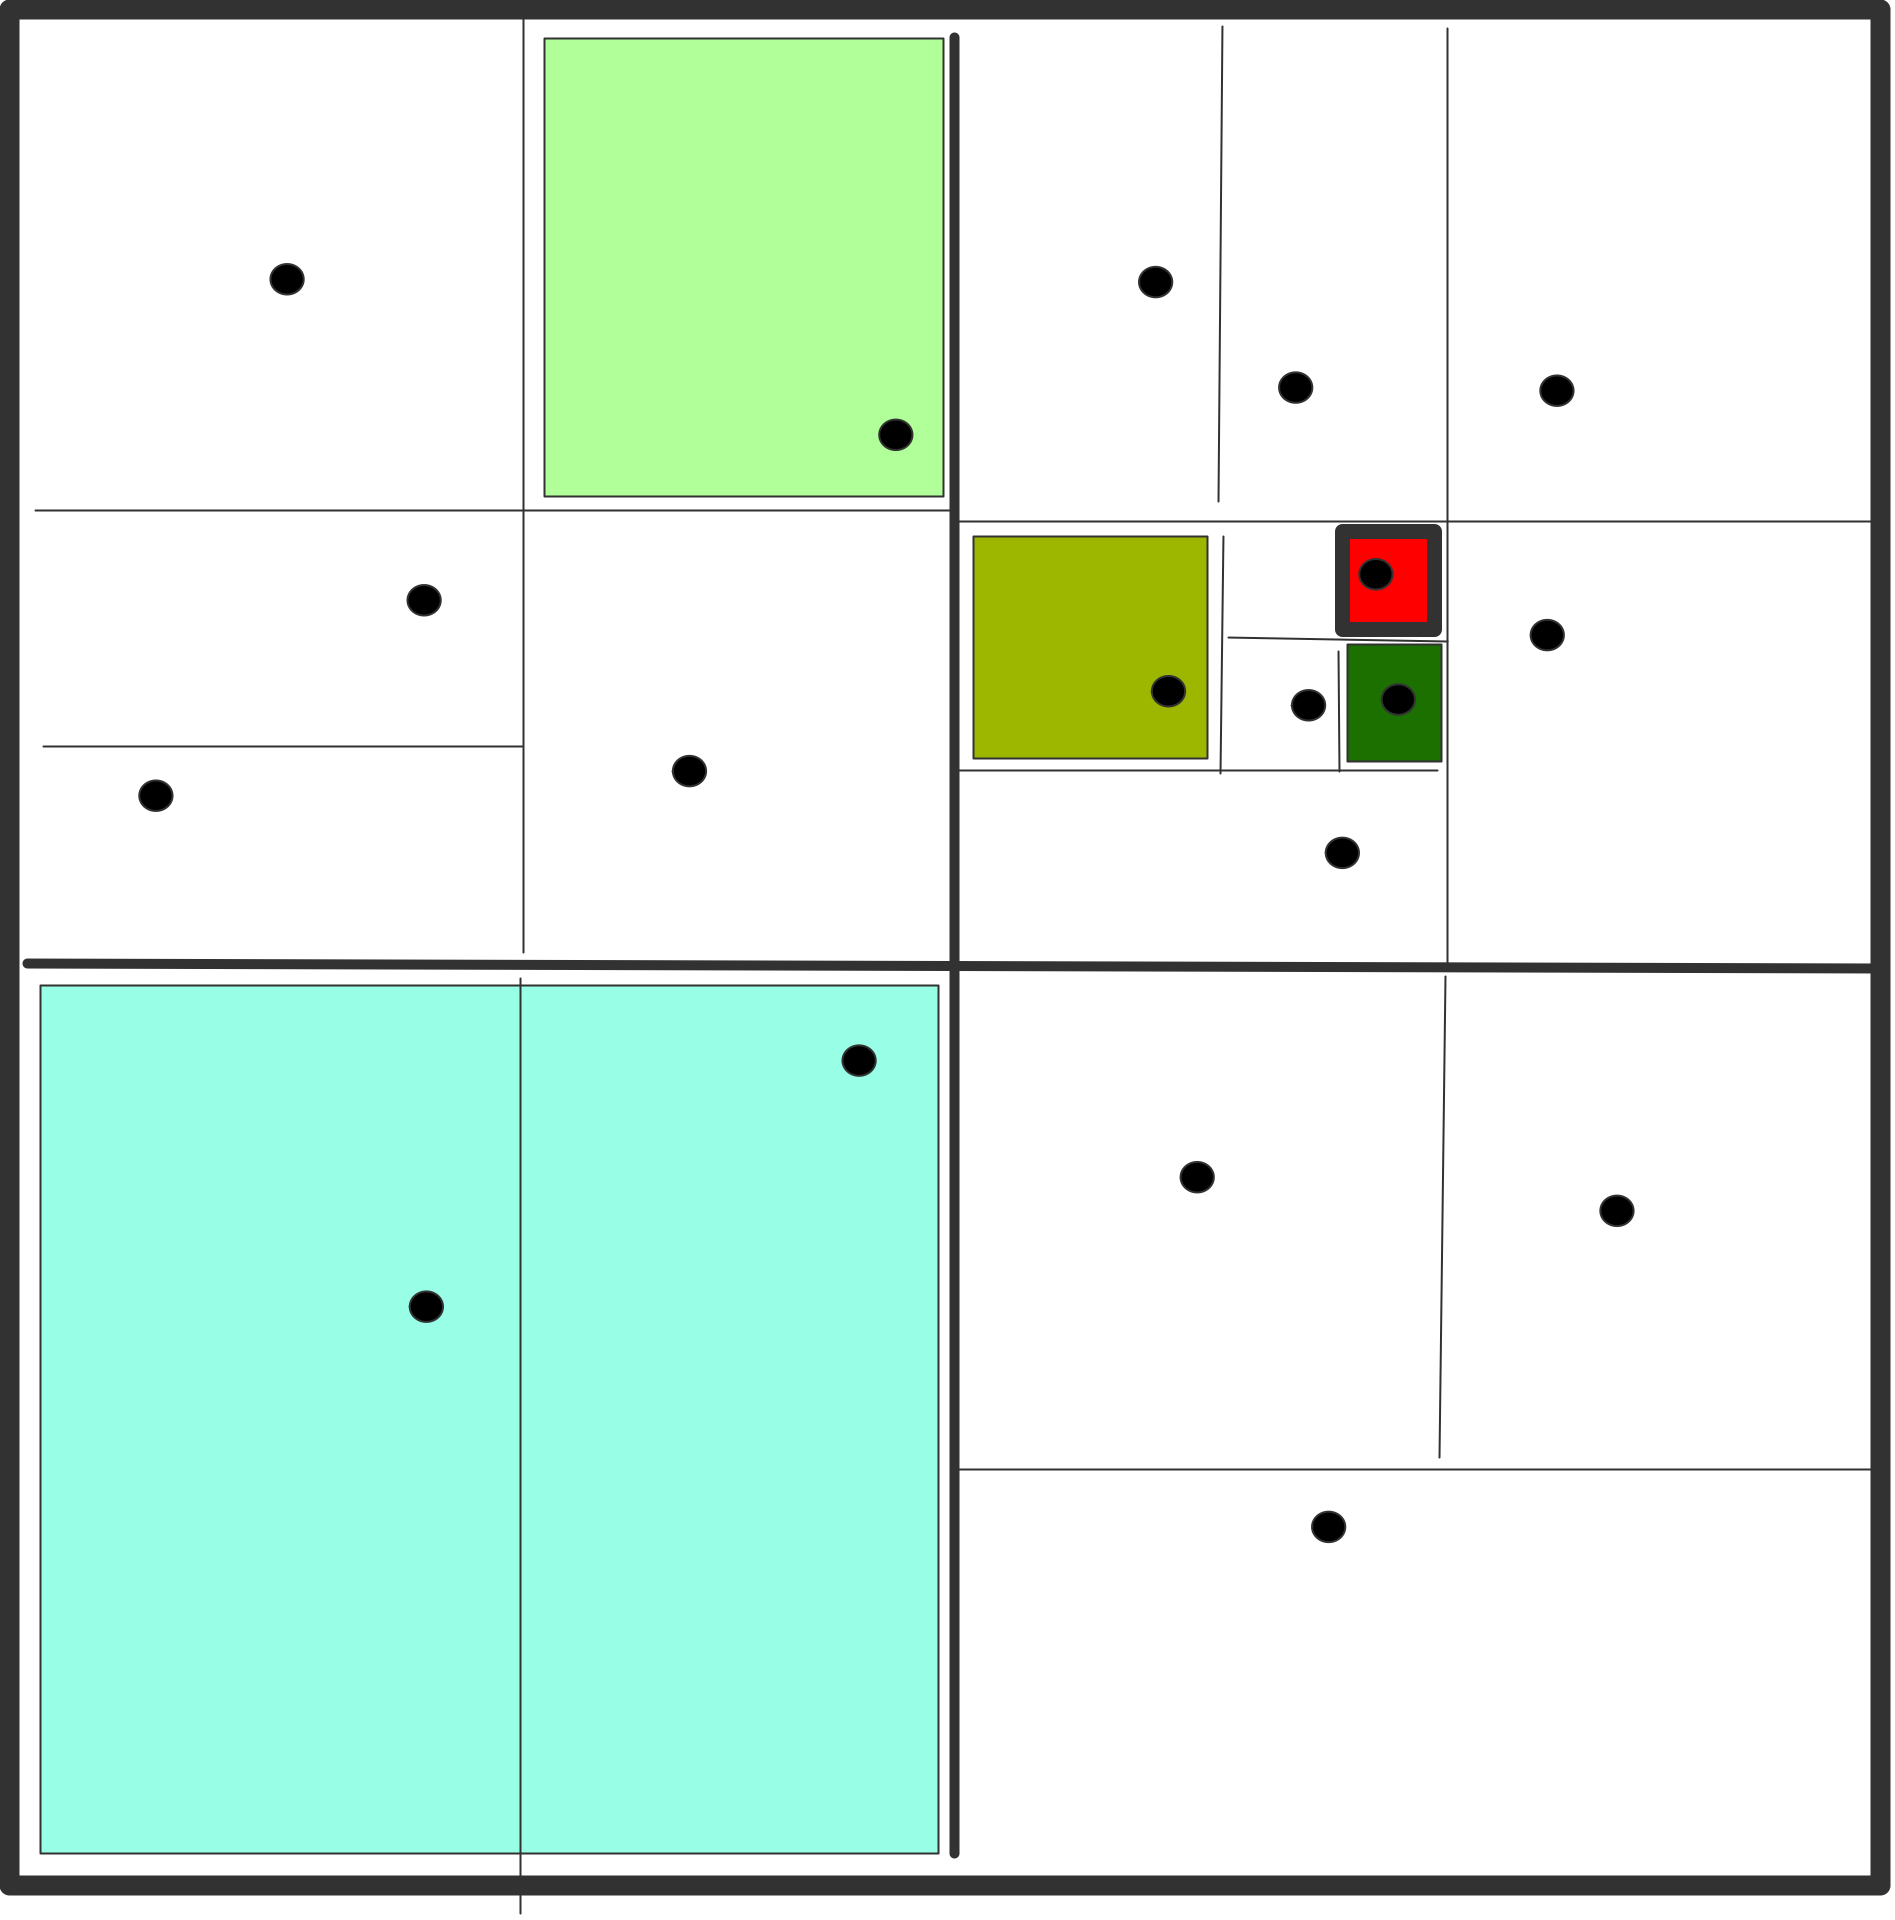
\includegraphics[scale=.08]{bh-quadrants-ratio}

  Clever algorithms: $O(N\log N)$, sometimes even~$O(N)$
\end{frame}

\sectionframe{Algorithm aspects}

\begin{frame}\frametitle{Linear algebra}
  \[\mathop{?}_x\colon Ax=b\]
  \begin{itemize}
  \item Inversion: $N^3$ operations, unstable
  \item Gaussian elimination: $N^3$ but lower constant, stable
  \item Sparse Gaussian elimination: $N^{3/2}$, hard to program
  \item Iterative methods: $N\cdot \kappa^{1/2}$, not always successful
  \item Multigrid: $O(N)$, very limited applicability.
  \end{itemize}
\end{frame}

\begin{frame}\frametitle{Sparse matrices}
  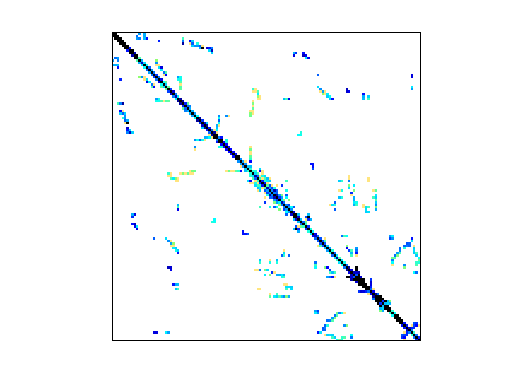
\includegraphics[scale=.5]{sparse_boeing}
\end{frame}

\begin{frame}{Permuting the matrix}
  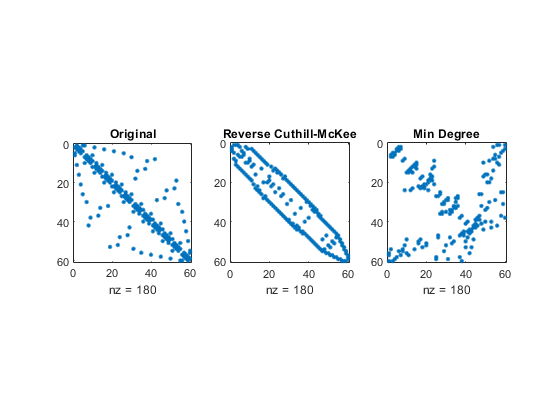
\includegraphics[scale=.6]{sparse_order}
\end{frame}

\sectionframe{The influence of your architecture}

\begin{frame}[containsverbatim]\frametitle{Fitting data to cache}
\begin{verbatim}
  for (j=0; j<size; j++)
    array[j] = 2.3*array[j]+1.2;
\end{verbatim}
  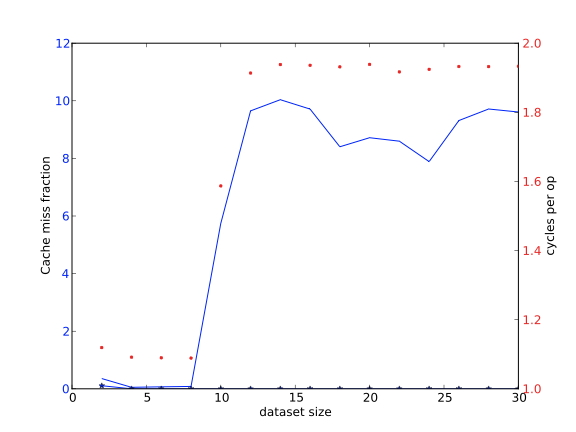
\includegraphics[scale=.35]{cacheoverflow}
\end{frame}

\begin{frame}\frametitle{Matrix-matrix product}
  Lots of small optimizations add up:

  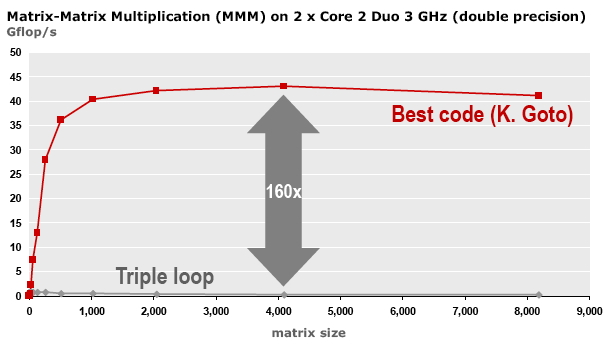
\includegraphics[scale=.5]{gemm}
\end{frame}

\begin{frame}\frametitle{Computer arithmetic}
    Computer numbers are not real numbers. If you don't pay attention
    to this you may lose you a race car, or a rocket
  \begin{multicols}{2}
    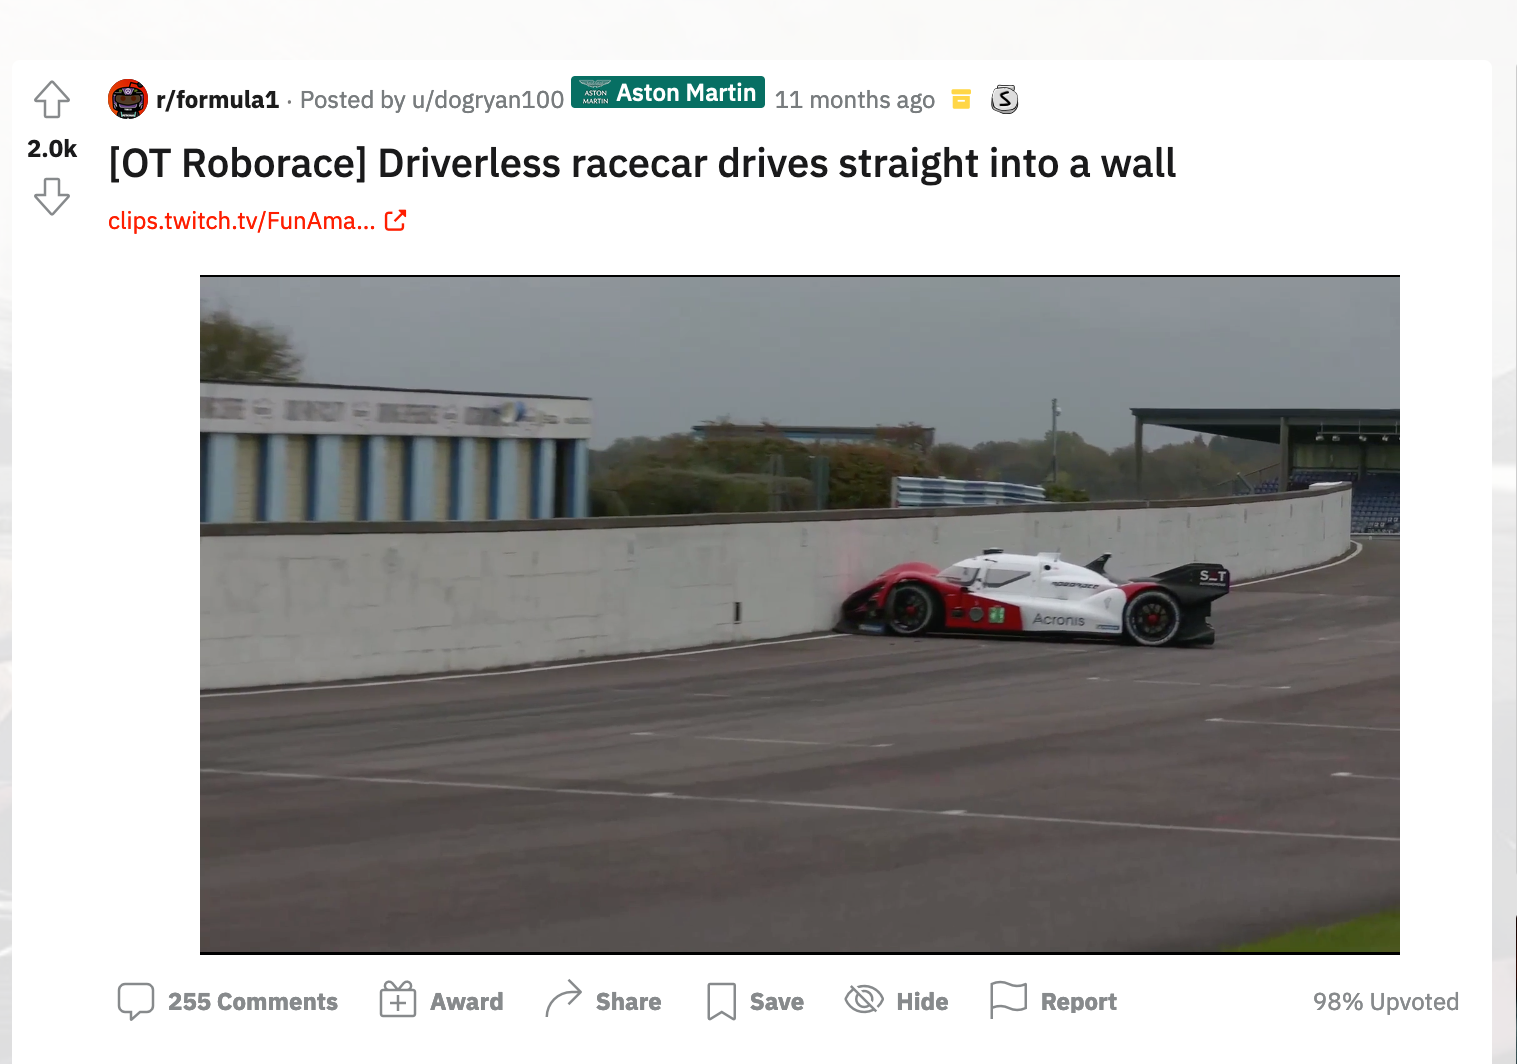
\includegraphics[scale=.12]{race-nan}
    \vfill\columnbreak
    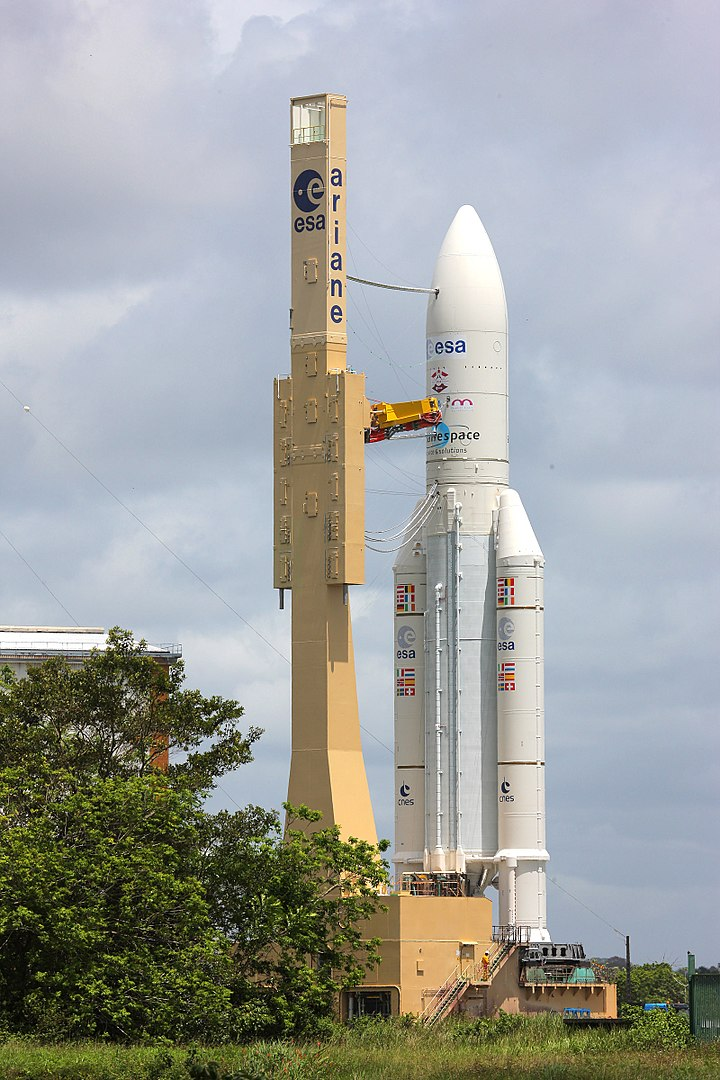
\includegraphics[scale=.15]{ariana5}
  \end{multicols}
\end{frame}

\sectionframe{So what is scientific computing about?}

\begin{frame}\frametitle{Between science and computing}
  \begin{itemize}
  \item Modeling
  \item Numerical analysis
  \item Linear algebra
  \item Computer architecture
  \item \ldots~and the interaction between any and all of these.
  \end{itemize}
\end{frame}

\end{document}

\begin{frame}\frametitle{}
  \begin{itemize}
  \item 
  \end{itemize}
\end{frame}

